\documentclass{beamer}
%% \documentclass[draft]{beamer} %% draft version

%% restrict generation of slides
%% \includeonlyframes{oligoarray,probesyn}

\mode<presentation>
{
  \usetheme{Bielefeld}
  \setbeamercovered{transparent}
}

\usepackage[english]{babel}
\usepackage[latin1]{inputenc}
\usepackage{graphicx}

\usepackage{lmodern}
\usepackage[T1]{fontenc}

\newcommand{\ignore}[1]{}

\title[Improving Microarray Layout: Pivot Partitioning] % (optional, use only with long paper titles)
{Improving the Layout of Oligonucleotide Microarrays: Pivot Partitioning}

%% \subtitle
%% {Include Only If Paper Has a Subtitle}

\author[S.~A.~de~Carvalho~Jr. (Universit\"at Bielefeld)] % (optional, use only with lots of authors)
{S\'ergio A. de Carvalho Jr.\inst{1,}\inst{2}\inst{,3} \and Sven Rahmann\inst{1,}\inst{2}}
% - Give the names in the same order as the appear in the paper.
% - Use the \inst{?} command only if the authors have different
%   affiliation.

\institute[Universit\"{a}t Bielefeld] % (optional, but mostly needed)
{
\inst{1}%
Algorithms and Statistics for Systems Biology, Genome Informatics,\\
Technische Fakult\"at, Universit\"at Bielefeld, Germany
\and
\inst{2}%
International NRW Graduate School in Bioinformatics and Genome Research
\and
\inst{3}%
Graduiertenkolleg Bioinformatik
}
% - Use the \inst command only if there are several affiliations.
% - Keep it simple, no one is interested in your street address.

\date[WABI 2006] % (optional, should be abbreviation of conference name)
{6th Workshop on Algorithms in Bioinformatics\\Z\"urich, Sep 2006}
% - Either use conference name or its abbreviation.
% - Not really informative to the audience, more for people (including
%   yourself) who are reading the slides online

% \subject{Theoretical Computer Science}
% This is only inserted into the PDF information catalog. Can be left
% out. 

% If you have a file called "university-logo-filename.xxx", where xxx
% is a graphic format that can be processed by latex or pdflatex,
% resp., then you can add a logo as follows:

% \pgfdeclareimage[height=0.5cm]{university-logo}{university-logo-filename}
% \logo{\pgfuseimage{university-logo}}

% Delete this, if you do not want the table of contents to pop up at
% the beginning of each subsection:
\AtBeginSubsection[]
{
  \begin{frame}<beamer>
    \frametitle{Outline}
    \tableofcontents[currentsection,hideallsubsections]
  \end{frame}
}

% If you wish to uncover everything in a step-wise fashion, uncomment
% the following command: 
%\beamerdefaultoverlayspecification{<+->}


\begin{document}

%%%%%%%%%%%%%%%%%%%%%%%%%%%%%%%%%%%%%%%%%%%%%%%%%%%%%%%%%%%%%%%%%%%%%%%%%%%%%%%%
\frame[plain]{

  \vspace*{0.4cm}
  \centerline{
    
\includegraphics[height=1.4cm]{aggi_logo.png}
    \hspace*{0.6cm}
    
\includegraphics[height=1.4cm]{gsbg_logo.png}
  }
  
  \titlepage
}

%%%%%%%%%%%%%%%%%%%%%%%%%%%%%%%%%%%%%%%%%%%%%%%%%%%%%%%%%%%%%%%%%%%%%%%%%%%%%%%%
\frame{\frametitle{Outline}

  \tableofcontents[hideallsubsections]

}

%% *****************************************************************************
\section[Introduction]{Introduction: Microarray Layout}
\subsection{Dummy}
%% *****************************************************************************

%%%%%%%%%%%%%%%%%%%%%%%%%%%%%%%%%%%%%%%%%%%%%%%%%%%%%%%%%%%%%%%%%%%%%%%%%%%%%%%%
\frame[label=oligoarray]{\frametitle{High-Density Oligonucleotide Microarrays}

  \centerline{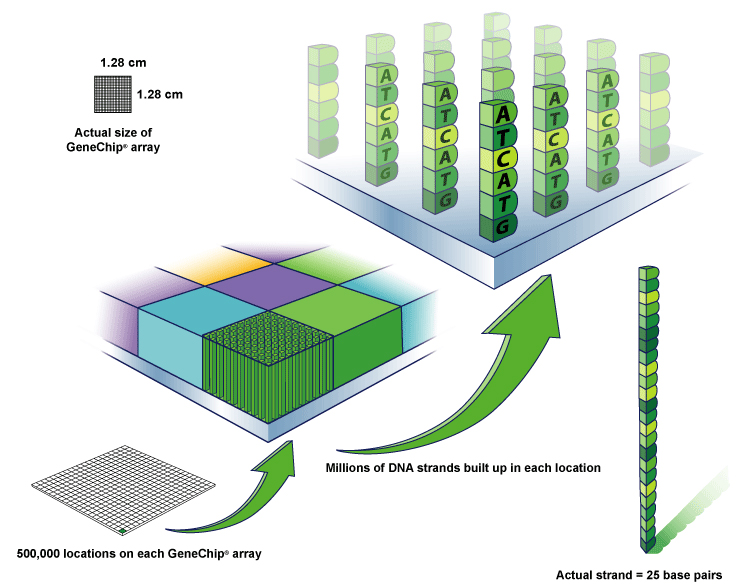
\includegraphics[height=0.9\textheight]{oligoarray.jpg}}
  \vspace*{-0.5cm}
  \centerline{\tiny{Source: Affymetrix, Inc.}}

}

%%%%%%%%%%%%%%%%%%%%%%%%%%%%%%%%%%%%%%%%%%%%%%%%%%%%%%%%%%%%%%%%%%%%%%%%%%%%%%%%
\frame[label=probesyn]{\frametitle{Probe Synthesis: Photolitographic Masks}

  \vspace*{-0.5cm}
  \flushright{\tiny{Source: Affymetrix, Inc.}}
  \centerline{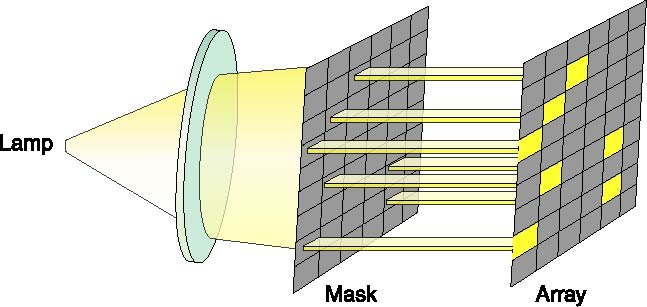
\includegraphics[height=0.5\textheight]{photolitography.jpg}}  

  \begin{itemize}
    \item Probes are synthesized on the chip in a series of \alert{steps}
    \item Each step appends a particular nucleotide to \alert{selected regions}
    \item Selection occurs by exposure to light
  \end{itemize}
}

%%%%%%%%%%%%%%%%%%%%%%%%%%%%%%%%%%%%%%%%%%%%%%%%%%%%%%%%%%%%%%%%%%%%%%%%%%%%%%%%
\frame[label=embed]{\frametitle{Deposition Sequence and Probe Embeddings}

  \vspace*{1cm}
  \centerline{
  \includegraphics<+>[width=\textwidth]{masks/chip.jpg}
  \includegraphics<+>[width=\textwidth]{masks/mask1.jpg}
  \includegraphics<+>[width=\textwidth]{masks/mask2.jpg}
  \includegraphics<+>[width=\textwidth]{masks/mask3.jpg}
  \includegraphics<+>[width=\textwidth]{masks/mask4.jpg}
  \includegraphics<+>[width=\textwidth]{masks/embed.jpg}
  \includegraphics<+>[width=\textwidth]{masks/leftmost.jpg}
  \includegraphics<+->[width=\textwidth]{masks/binary.jpg}
  }
  \onslide+<7>{
    \hspace{7cm}
    \alert{Left-most embedding!}
  }

}

%%%%%%%%%%%%%%%%%%%%%%%%%%%%%%%%%%%%%%%%%%%%%%%%%%%%%%%%%%%%%%%%%%%%%%%%%%%%%%%%
\frame[label=problem]{\frametitle{Problem: Unintended Illumination}

  \begin{columns}
  
    \begin{column}{0.45\textwidth}
      \centerline{
        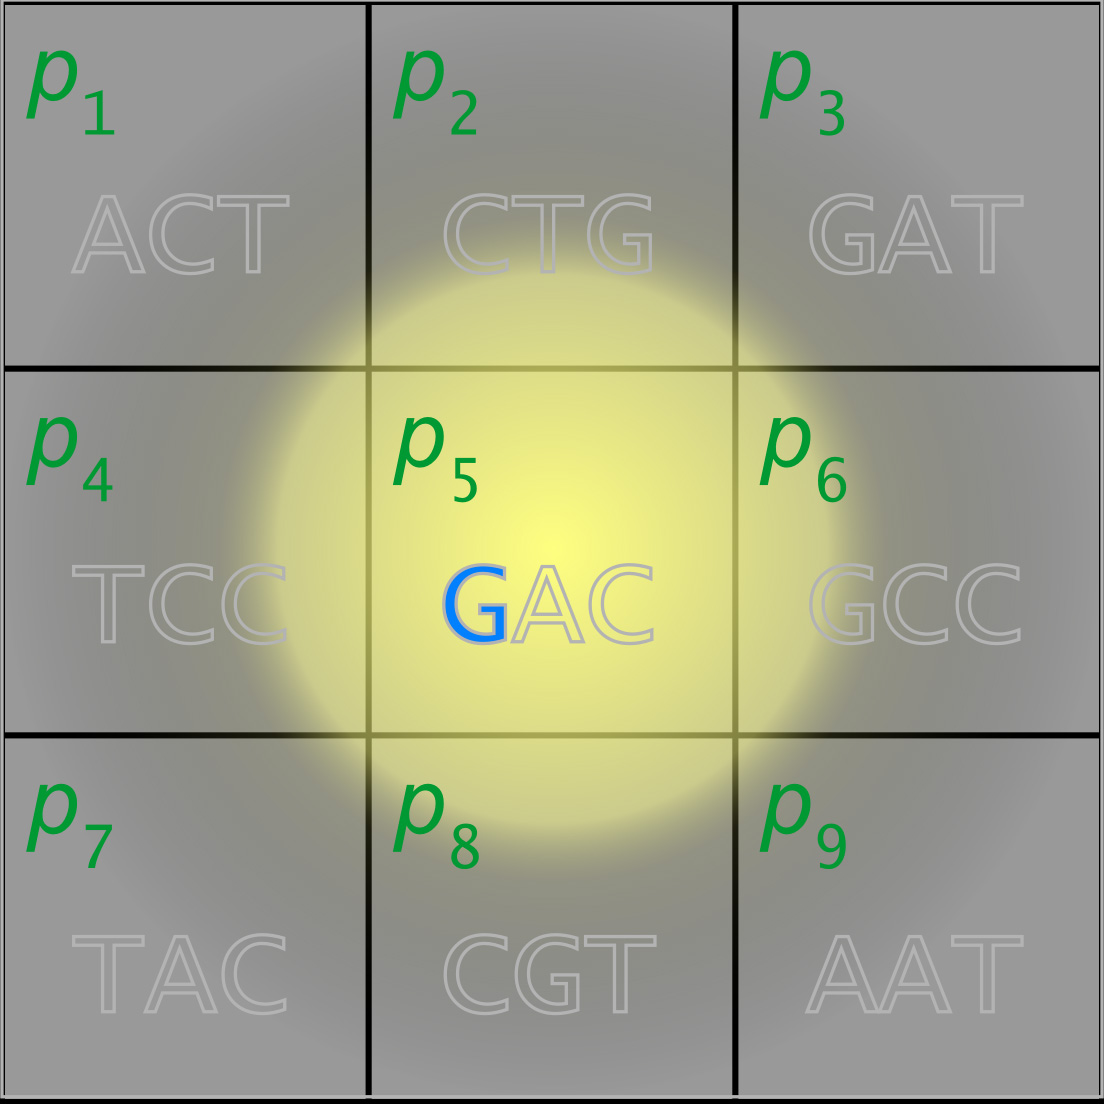
\includegraphics[width=\textwidth]{pics/straylight.jpg}
      }
    \end{column}
    
    \begin{column}{0.55\textwidth}
      \begin{itemize}
        \item \alert{Untargeted spots} can be accidentally activated
        \begin{itemize}
          \item Diffraction of light
          \item Internal reflection
        \end{itemize}
        \item Production of defective probes
        \item More likely near the \alert{borders} between masked and unmasked
              spots: \alert{border conflict}
      \end{itemize}
    \end{column}
    
  \end{columns}
  
  \begin{block}{Border Length Minimization Problem (Hannenhalli et al., 2002)}
    \begin{itemize}
      \item Find arrangement (and embeddings) with minimum number of border
            conflicts
    \end{itemize}
  \end{block}

}

%% *****************************************************************************
\section[Conflict Index]{Conflict Index Evaluation Model}
\subsection{Dummy}
%% *****************************************************************************

%%%%%%%%%%%%%%%%%%%%%%%%%%%%%%%%%%%%%%%%%%%%%%%%%%%%%%%%%%%%%%%%%%%%%%%%%%%%%%%%
\frame{\frametitle{Conflict Index: Motivation}

  \begin{itemize}
    \item Border Length measures the quality of a particular mask
    \begin{itemize}
      \item We are more interested in a \alert{per-probe} measure
    \end{itemize}
    \item Practical considerations need to be taken into account:
    \begin{itemize}
      \item[a)] Stray light might activate probes that are as far as \alert{three
                cells away} from the targeted spot
      \item[b)] Imperfections produced \alert{in the middle} of a probe are more
                harmful than in its extremities
    \end{itemize}
  \end{itemize}
  
  \begin{block}{Conflict Index of a probe $p$}
    \footnotesize{
    \[
    \mathcal{C}(p) := \sum_{t=1}^{T} \Bigl( \omega(p,t) \sum_{p'} \delta(p,p',t) \Bigr),
    \]
    where $\delta(p,p',t)$ are \alert{distance-dependent} weights (a) and
    $\omega(p,t)$ are \alert{position-dependent} weights (b) defined as follows.
    }
  \end{block}
}

%%%%%%%%%%%%%%%%%%%%%%%%%%%%%%%%%%%%%%%%%%%%%%%%%%%%%%%%%%%%%%%%%%%%%%%%%%%%%%%%
\frame{\frametitle{Conflict Index: Definition}

  \begin{columns}
  
    \begin{column}{0.45\textwidth}
      \begin{block}{Conflict Index of a probe $p$}
        \footnotesize{
        \[
        \mathcal{C}(p) := \sum_{t=1}^{T} \Bigl( \omega(p,t) \sum_{p'} \delta(p,p',t) \Bigr)
        \]
        }
      \end{block}
    \end{column}
    
    \begin{column}{0.45\textwidth}
      \begin{figure}
        \centerline{
        \begin{picture}(165,55)
        %% \put(0,0){\framebox(165,55){}}
        \put(-5,0){\makebox(165,55){
        \begin{minipage}{160pt}
        \centerline{
        \tiny{
        \begin{tabular}{|c|c|c|c|c|c|c|c|} \hline
        0.06 & 0.08 & 0.10 & 0.11 & 0.10 & 0.08 & 0.06 \\ \hline
        0.08 & 0.13 & 0.20 & 0.25 & 0.20 & 0.13 & 0.08 \\ \hline
        0.10 & 0.20 & 0.50 & 1.00 & 0.50 & 0.20 & 0.10 \\ \hline
        0.11 & 0.25 & 1.00 & \alert{$p$} & 1.00 & 0.25 & 0.11 \\ \hline
        0.10 & 0.20 & 0.50 & 1.00 & 0.50 & 0.20 & 0.10 \\ \hline
        0.08 & 0.13 & 0.20 & 0.25 & 0.20 & 0.13 & 0.08 \\ \hline
        0.06 & 0.08 & 0.10 & 0.11 & 0.10 & 0.08 & 0.06 \\ \hline
        \end{tabular}}}
        \end{minipage}}}
        \end{picture}}
      \end{figure}
    \end{column}
    
  \end{columns}
  
  \begin{block}{a) Distance-dependent weights $\delta(p,p',t)$}
    \footnotesize{
    \[
    \delta(p,p',t) :=
    \left\{
    \begin{array}{ll}
    (d(p,p'))^{-2} & \mbox{if $p'$ is unmasked at step $t$}, \\
                 0 & \mbox{otherwise}, \\
    \end{array}
    \right.
    \]
    %%
    where $d(p,p')$ is the Euclidean distance between the spots of~$p$ and~$p'$.
    }
  \end{block}
  
}

%%%%%%%%%%%%%%%%%%%%%%%%%%%%%%%%%%%%%%%%%%%%%%%%%%%%%%%%%%%%%%%%%%%%%%%%%%%%%%%%
\frame{\frametitle{Conflict Index: Definition}

  \begin{columns}
  
    \begin{column}{0.45\textwidth}
      \begin{block}{Conflict Index of a probe $p$}
        \footnotesize{
        \[
        \mathcal{C}(p) := \sum_{t=1}^{T} \Bigl( \omega(p,t) \sum_{p'} \delta(p,p',t) \Bigr)
        \]
        }
      \end{block}
    \end{column}
    
    \begin{column}{0.45\textwidth}
      \centerline{
        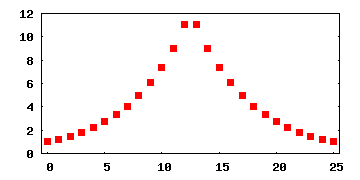
\includegraphics[width=1.25\textwidth]{pics/position_weights.png}
      }
    \end{column}
    
  \end{columns}

  \begin{block}{b) Position-dependent weights $\omega(p,t)$}
    \footnotesize{
    \[
    \omega(p,t) :=
    \left\{
    \begin{array}{ll}
    c \cdot \exp{\left(\theta \cdot \lambda(p,t)\right)} & \mbox{if $p$ is masked at step $t$}, \\
    0 & \mbox{otherwise}, \\
    \end{array}
    \right.
    \]
    %%
    where $c>0$ and $\theta>0$ are constants,
    %%
    \[
    \lambda(p,t) := 1 + \min(b_{p,t},\ell_{p} - b_{p,t}),
    \]
    %%
    $b_{p,t}$ denotes the number of nucleotides synthesized up to and
    including step~$t$, and $\ell_{p}$ is the length of probe~$p$.
    }
  \end{block}

}

%% *****************************************************************************
\section[Pivot Partitioning]{Pivot Partitioning Algorithm}
\subsection{Dummy}
%% *****************************************************************************

%%%%%%%%%%%%%%%%%%%%%%%%%%%%%%%%%%%%%%%%%%%%%%%%%%%%%%%%%%%%%%%%%%%%%%%%%%%%%%%%
\frame{\frametitle{Previous work}
}

%% *****************************************************************************
\section*{Summary}
\subsection*{Dummy}
%% *****************************************************************************

%%%%%%%%%%%%%%%%%%%%%%%%%%%%%%%%%%%%%%%%%%%%%%%%%%%%%%%%%%%%%%%%%%%%%%%%%%%%%%%%
\frame{\frametitle{Summary}
}

%%%%%%%%%%%%%%%%%%%%%%%%%%%%%%%%%%%%%%%%%%%%%%%%%%%%%%%%%%%%%%%%%%%%%%%%%%%%%%%%
\begin{frame}{Thanks!}

  \centerline{
    
\includegraphics[height=1.4cm]{aggi_logo.png}
    \hspace*{0.6cm}
    
\includegraphics[height=1.4cm]{gsbg_logo.png}
  }

  \begin{itemize}
    \item Prof. Dr. Jens Stoye
    \item Prof. Dr. Robert Giegerich
    \item AG Genominformatik
    \item Graduiertenkolleg Bioinformatik
    \item Graduate School in Bioinformatics and Genome Research
    
    \vskip0pt plus.5fill
    
    \item ...and \alert{thank you} for your attention!
  \end{itemize}
  
\end{frame}

\end{document}
